\subsection{Trilateration}

\subsubsection*{Rechnerische Lösung}

\subsubsection*{Graphische Validierung}

Die errechnete Lösung kann zudem recht leicht graphisch verifiziert werden. Dazu werden zuerst die Punkte, die die Standorte der APs darstellen geplottet (hier in GeoGebra). Anschließend werden die 4 Gleichungen hinzugefügt. Wie zu erwarten, entsteht dadurch für jeden AP ein Kreis mit diesem AP als Mittelpunkt, die Durchmesser sind aber jeweils verschieden.

Auch wenn es auf den ersten Blick so aussieht, als ob es eine exakte Lösung gäbe: Spätestens beim Heranzoomen wird klar, dass sich an keinem einzigen Punkt auch nur drei der vier Kreise schneiden.

\begin{figure}[H]
    \centering
    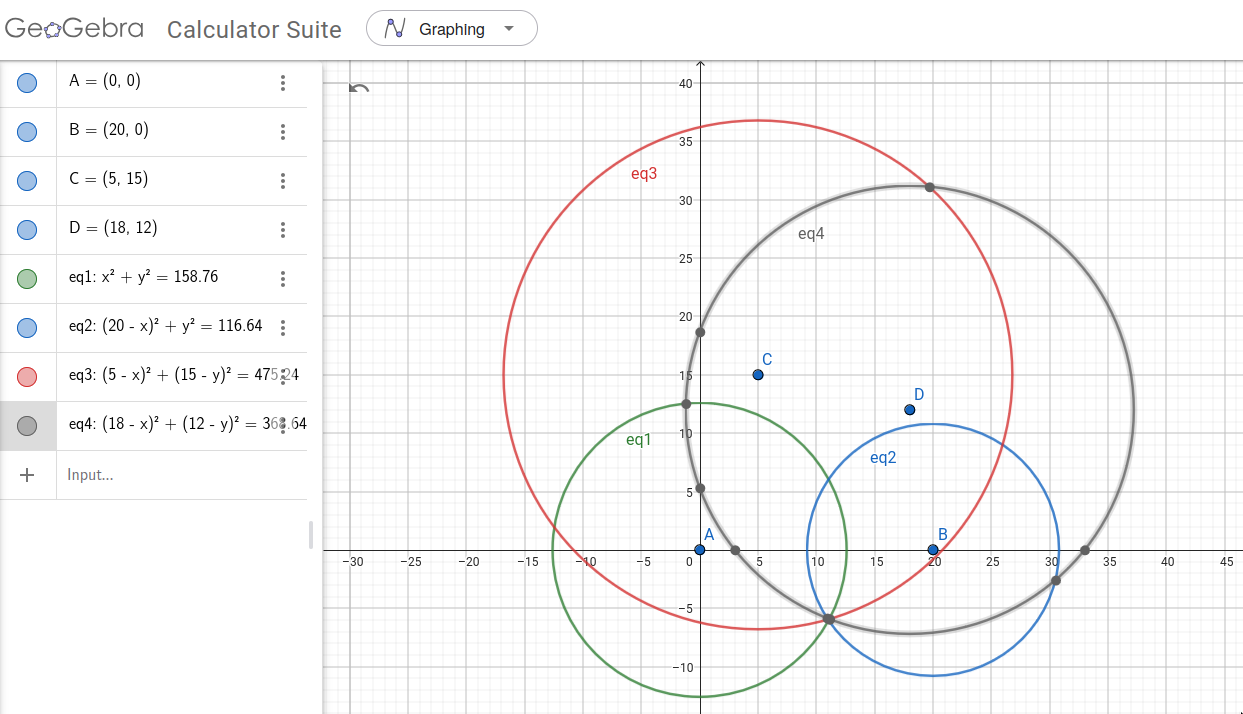
\includegraphics[width=0.5\textwidth]{figures/geogebra/screen_2.png}
    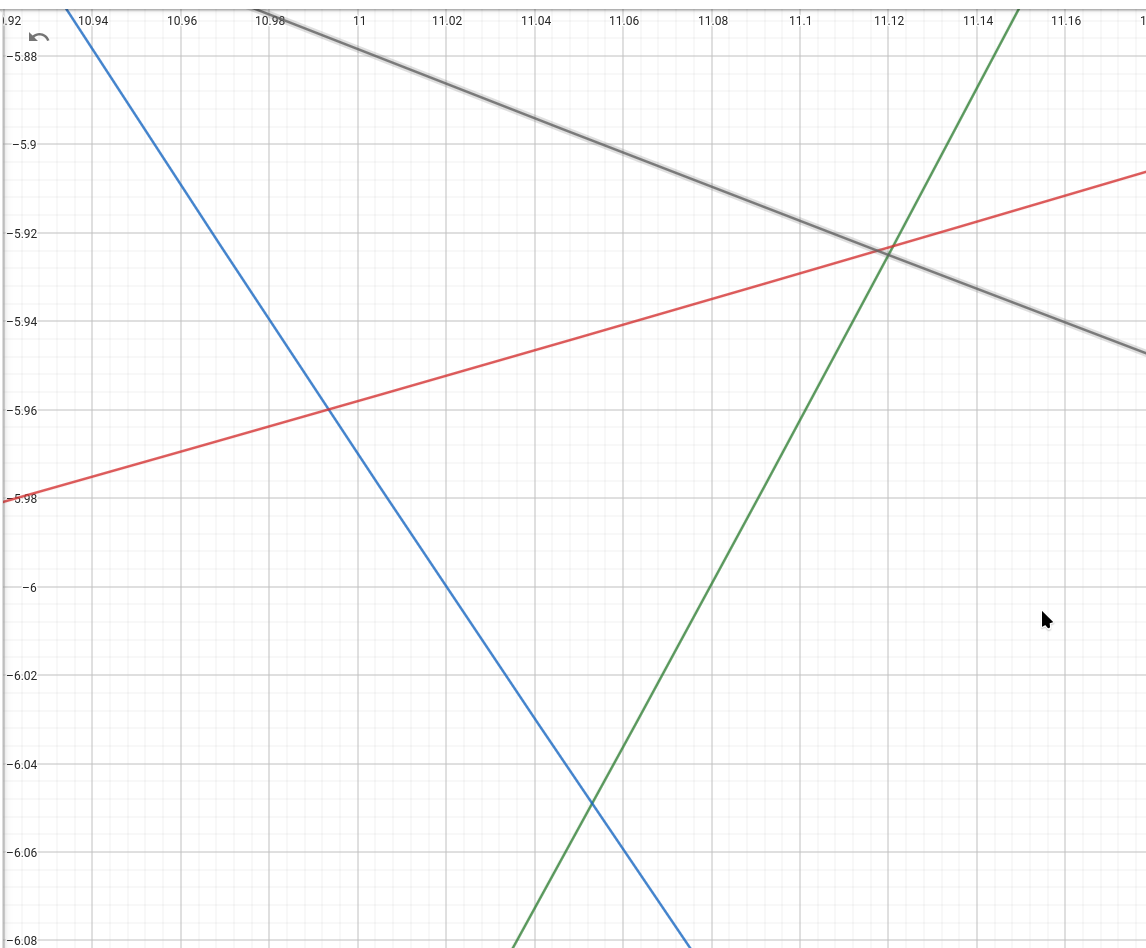
\includegraphics[width=0.4\textwidth]{figures/geogebra/screen_3.png}
    \caption{Graphische Validierung der errechneten Lösung mit GeoGebra. Links sind die konzentrischen Kreise um die vier APs zu sehen, rechts der vermeintliche Schnittpunkt der Kreise.}
    \label{geogebra}
\end{figure}